\section{Sơ đồ Lược đồ Logic (Logical Schema Diagram)}

Lược đồ logic được xây dựng dựa trên mô hình ERD đã hoàn thiện và tập phụ thuộc hàm được xác định ở các mục trước. Sơ đồ thể hiện các quan hệ, thuộc tính, khóa chính (Primary Key - PK), khóa ngoại (Foreign Key - FK) và bản số của các mối quan hệ.

Trong mô hình OctaPoint, \texttt{CREDIT} là ví điểm dùng chung của một \texttt{CUSTOMER} trong phạm vi một \texttt{TENANT}. Vì vậy, \texttt{CREDIT} tham chiếu đến \texttt{CUSTOMER} và \texttt{TENANT}, không tham chiếu trực tiếp đến \texttt{MERCHANT}.

Bên cạnh đó, \texttt{CAMPAIGN} thuộc về một \texttt{TENANT}. Một Campaign có thể áp dụng cho nhiều Merchant và một Merchant có thể tham gia nhiều Campaign. Do đó, mối quan hệ M:N giữa \texttt{CAMPAIGN} và \texttt{MERCHANT} được phân rã thông qua bảng trung gian \texttt{CAMPAIGN\_MERCHANT}.

\begin{figure}[H]
    \centering
    \resizebox{\textwidth}{!}{
    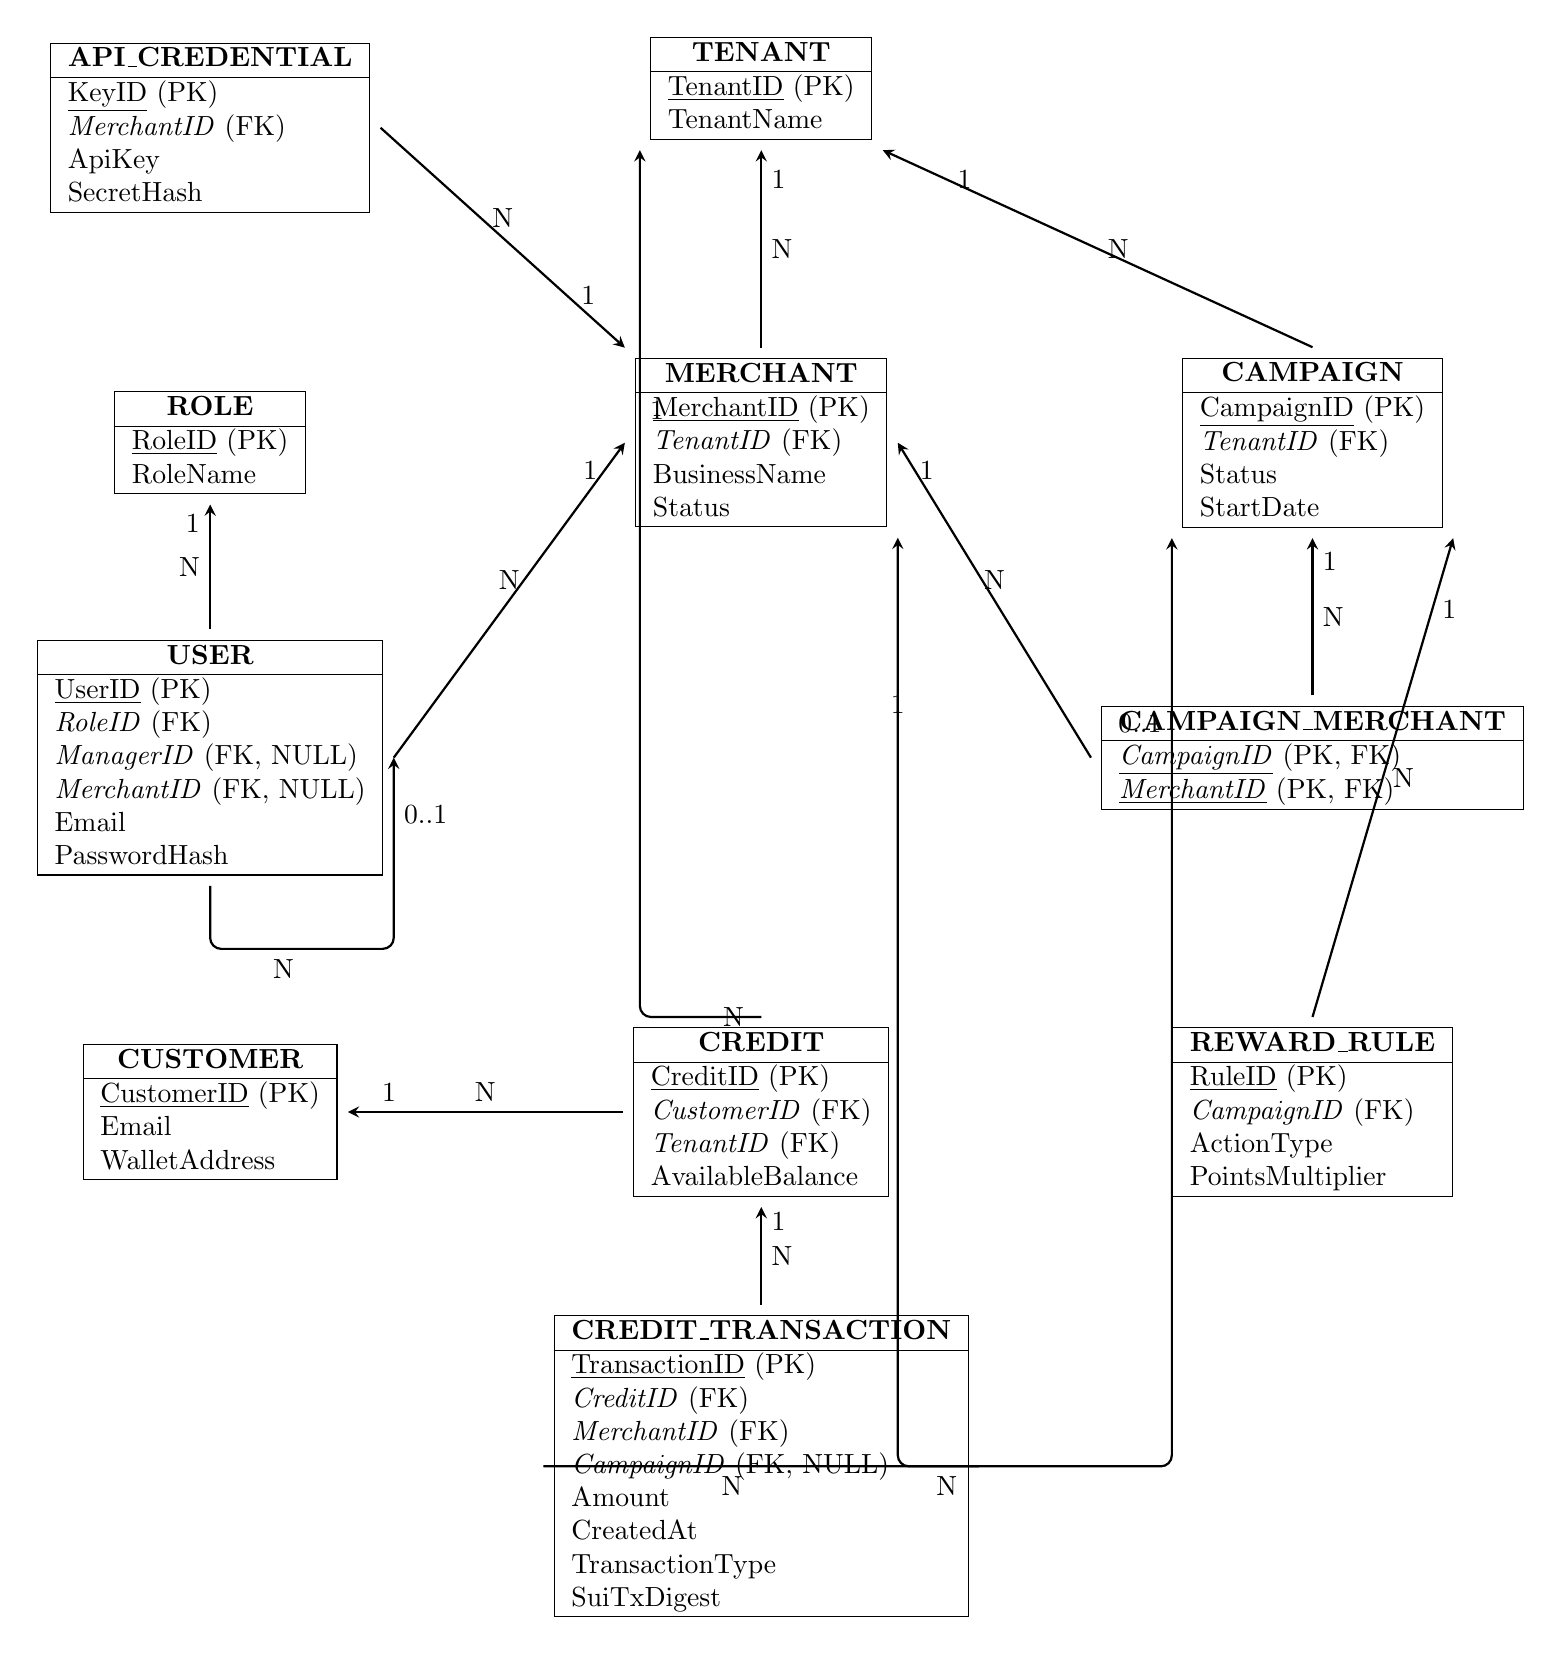
\begin{tikzpicture}[>=stealth, thick]

        % ========================================================
        % TENANT
        % ========================================================
        \node (tenant) at (0,6) {
            \begin{tabular}{|l|}
            \hline
            \multicolumn{1}{|c|}{\textbf{TENANT}} \\ \hline
            \underline{TenantID} (PK) \\
            TenantName \\ \hline
            \end{tabular}
        };

        % ========================================================
        % MERCHANT
        % ========================================================
        \node (merchant) at (0,1.5) {
            \begin{tabular}{|l|}
            \hline
            \multicolumn{1}{|c|}{\textbf{MERCHANT}} \\ \hline
            \underline{MerchantID} (PK) \\
            \textit{TenantID} (FK) \\
            BusinessName \\
            Status \\ \hline
            \end{tabular}
        };

        % ========================================================
        % ROLE
        % ========================================================
        \node (role) at (-7,1.5) {
            \begin{tabular}{|l|}
            \hline
            \multicolumn{1}{|c|}{\textbf{ROLE}} \\ \hline
            \underline{RoleID} (PK) \\
            RoleName \\ \hline
            \end{tabular}
        };

        % ========================================================
        % USER
        % ========================================================
        \node (user) at (-7,-2.5) {
            \begin{tabular}{|l|}
            \hline
            \multicolumn{1}{|c|}{\textbf{USER}} \\ \hline
            \underline{UserID} (PK) \\
            \textit{RoleID} (FK) \\
            \textit{ManagerID} (FK, NULL) \\
            \textit{MerchantID} (FK, NULL) \\
            Email \\
            PasswordHash \\ \hline
            \end{tabular}
        };

        % ========================================================
        % API CREDENTIAL
        % ========================================================
        \node (api) at (-7,5.5) {
            \begin{tabular}{|l|}
            \hline
            \multicolumn{1}{|c|}{\textbf{API\_CREDENTIAL}} \\ \hline
            \underline{KeyID} (PK) \\
            \textit{MerchantID} (FK) \\
            ApiKey \\
            SecretHash \\ \hline
            \end{tabular}
        };

        % ========================================================
        % CAMPAIGN
        % ========================================================
        \node (campaign) at (7,1.5) {
            \begin{tabular}{|l|}
            \hline
            \multicolumn{1}{|c|}{\textbf{CAMPAIGN}} \\ \hline
            \underline{CampaignID} (PK) \\
            \textit{TenantID} (FK) \\
            Status \\
            StartDate \\ \hline
            \end{tabular}
        };

        % ========================================================
        % CAMPAIGN MERCHANT
        % ========================================================
        \node (cm) at (7,-2.5) {
            \begin{tabular}{|l|}
            \hline
            \multicolumn{1}{|c|}{\textbf{CAMPAIGN\_MERCHANT}} \\ \hline
            \underline{\textit{CampaignID}} (PK, FK) \\
            \underline{\textit{MerchantID}} (PK, FK) \\ \hline
            \end{tabular}
        };

        % ========================================================
        % CUSTOMER
        % ========================================================
        \node (customer) at (-7,-7) {
            \begin{tabular}{|l|}
            \hline
            \multicolumn{1}{|c|}{\textbf{CUSTOMER}} \\ \hline
            \underline{CustomerID} (PK) \\
            Email \\
            WalletAddress \\ \hline
            \end{tabular}
        };

        % ========================================================
        % CREDIT
        % ========================================================
        \node (credit) at (0,-7) {
            \begin{tabular}{|l|}
            \hline
            \multicolumn{1}{|c|}{\textbf{CREDIT}} \\ \hline
            \underline{CreditID} (PK) \\
            \textit{CustomerID} (FK) \\
            \textit{TenantID} (FK) \\
            AvailableBalance \\ \hline
            \end{tabular}
        };

        % ========================================================
        % REWARD RULE
        % ========================================================
        \node (rule) at (7,-7) {
            \begin{tabular}{|l|}
            \hline
            \multicolumn{1}{|c|}{\textbf{REWARD\_RULE}} \\ \hline
            \underline{RuleID} (PK) \\
            \textit{CampaignID} (FK) \\
            ActionType \\
            PointsMultiplier \\ \hline
            \end{tabular}
        };

        % ========================================================
        % CREDIT TRANSACTION
        % ========================================================
        \node (transaction) at (0,-11.5) {
            \begin{tabular}{|l|}
            \hline
            \multicolumn{1}{|c|}{\textbf{CREDIT\_TRANSACTION}} \\ \hline
            \underline{TransactionID} (PK) \\
            \textit{CreditID} (FK) \\
            \textit{MerchantID} (FK) \\
            \textit{CampaignID} (FK, NULL) \\
            Amount \\
            CreatedAt \\
            TransactionType \\
            SuiTxDigest \\ \hline
            \end{tabular}
        };

        % ========================================================
        % RELATIONSHIPS
        % ========================================================

        % TENANT - MERCHANT
        \draw[->]
        (merchant.north)
        -- node[right] {N}
        node[right, pos=0.85] {1}
        (tenant.south);

        % TENANT - CAMPAIGN
        \draw[->]
        (campaign.north)
        -- node[right] {N}
        node[right, pos=0.85] {1}
        (tenant.south east);

        % ROLE - USER
        \draw[->]
        (user.north)
        -- node[left] {N}
        node[left, pos=0.85] {1}
        (role.south);

        % MERCHANT - USER
        \draw[->]
        (user.east)
        -- node[above] {N}
        node[above, pos=0.85] {1}
        (merchant.west);

        % MERCHANT - API
        \draw[->]
        (api.east)
        -- node[above] {N}
        node[above, pos=0.85] {1}
        (merchant.north west);

        % CAMPAIGN - CAMPAIGN_MERCHANT
        \draw[->]
        (cm.north)
        -- node[right] {N}
        node[right, pos=0.85] {1}
        (campaign.south);

        % MERCHANT - CAMPAIGN_MERCHANT
        \draw[->]
        (cm.west)
        -- node[above] {N}
        node[above, pos=0.85] {1}
        (merchant.east);

        % CAMPAIGN - REWARD RULE
        \draw[->]
        (rule.north)
        -- node[right] {N}
        node[right, pos=0.85] {1}
        (campaign.south east);

        % CUSTOMER - CREDIT
        \draw[->]
        (credit.west)
        -- node[above] {N}
        node[above, pos=0.85] {1}
        (customer.east);

        % TENANT - CREDIT
        \draw[->, rounded corners]
        (credit.north)
        -| node[pos=0.2, right] {N}
        node[pos=0.85, right] {1}
        (tenant.south west);

        % CREDIT - TRANSACTION
        \draw[->]
        (transaction.north)
        -- node[right] {N}
        node[right, pos=0.85] {1}
        (credit.south);

        % MERCHANT - TRANSACTION
        \draw[->, rounded corners]
        (transaction.east)
        -| node[pos=0.2, below] {N}
        node[pos=0.9, above] {1}
        (merchant.south east);

        % CAMPAIGN - TRANSACTION
        \draw[->, rounded corners]
        (transaction.west)
        -| node[pos=0.15, below] {N}
        node[pos=0.9, left] {0..1}
        (campaign.south west);

        % USER SELF RELATIONSHIP
        \draw[->, rounded corners]
        (user.south)
        -- ++(0,-0.8)
        -| node[pos=0.2, below] {N}
        node[pos=0.85, right] {0..1}
        (user.east);

    \end{tikzpicture}
    }

    \caption{Sơ đồ Lược đồ Logic hệ thống OctaPoint CaaS}
    \label{fig:sodo_logic_tikz}
\end{figure}

\textit{Ghi chú:} Các đường liên kết thể hiện quan hệ giữa khóa ngoại và khóa chính của các quan hệ. Nhãn ``1'' và ``N'' biểu diễn bản số của các mối quan hệ.

Mỗi \texttt{CREDIT} thuộc về một \texttt{CUSTOMER} và một \texttt{TENANT}. Ràng buộc \texttt{UNIQUE(CustomerID,TenantID)} bảo đảm một khách hàng chỉ có tối đa một Credit trong cùng một Tenant.

Mối quan hệ giữa \texttt{CAMPAIGN} và \texttt{MERCHANT} là M:N và được phân rã thông qua \texttt{CAMPAIGN\_MERCHANT}.

Trong \texttt{CREDIT\_TRANSACTION}, \texttt{MerchantID} bắt buộc để ghi nhận Merchant nơi giao dịch phát sinh, trong khi \texttt{CampaignID} có thể NULL vì giao dịch không nhất thiết phải thuộc một Campaign.

\texttt{ManagerID} trong \texttt{USER} là khóa ngoại tự tham chiếu đến \texttt{UserID}. Một User có thể không có Manager hoặc có một Manager trực tiếp.
